\section{Spherical Harmonics Transform}
In the variable phase method, we must find the spherical 
harmonics transform, i.e. the spherical moments, of the 
potential. To find these moments, we will have to become
intimate with the spherical harmonics. 

\subsection{Definition of the scalar and vector spherical harmonics}
While there is a number of ways to introduce the spherical harmonics, 
we will take the top to bottom approach: from the general to the specific. 
In all generality, spherical harmonics are solutions of the equation
  \begin{equation}
    \left[\nabla^2_\Omega+\ell(\ell+1)\right]Y^{\ell S}_{jm}(\theta,\varphi)=0
  \end{equation}
where $Y_{jm}^{\ell S}$ is actually a \textit{tensor} spherical harmonic. 
It describes the angular distribution and polarization of spin-$S$ particles 
with angular momentum $j$, projection $m$ and orbital angular momentum $\ell$ \cite{VAR1988}.
While the study of particles with arbitrary spin $S$ is interesting in its own right,
we will concentrate on the case of particles of spin-$1$ and their scalar approximation
(spin-$0$). Since the values of $\ell$ range from $|J-S|$ to $J+S$, the 
spin-$0$ case reduces to the usual scalar spherical harmonics while the spin-$1$
case are the \textit{vector} spherical harmonics. As said in the main text, they 
can be formed by a superposition of scalar spherical harmonics of the form
  \begin{equation}
    \bo{Y}_{jm}^\ell(\theta,\varphi)=\sum_{m',\sigma}C_{lm',1\sigma}^{jm}Y_\ell^{m'}(\theta,\varphi)\hat{\bo{e}}_\sigma
  \end{equation}
The numerical evaluation of these functions are then contingent on the evaluation of the
scalar spherical harmonics and the Clebsch-Gordan coefficients. The first was covered in the 
previous appendix and we will soon tend to the second. 

The scalar spherical harmonics can simply be written as
  \begin{equation}
   Y_{\ell}^m(\theta,\varphi) = P_\ell^m(\cos\theta)e^{im\varphi}
  \end{equation}
where $P_\ell^m$ is the normalized version of the associated 
Legendre polynomials \cite{PRE2007}. They are related to
the usual Legendre polynomials $\widetilde{P}_\ell^m$ through
  \begin{equation}
    P_\ell^m(x) = \sqrt{\frac{2\ell+1}{4\pi}\frac{(\ell-m)!}{(\ell+m)!}}\widetilde{P}_\ell^m(x)
  \end{equation}
To numerically evaluate the spherical harmonics, then, we must safely 
evaluate the associated Legendre polynomials. One of the only 
stable recurrence relation is \cite{PRE2007}
  
  \begin{equation}
   P_\ell^m(x)=\sqrt{\frac{4l^2-1}{l^2-m^2}}\left[xP_{\ell-1}^m(x)-\sqrt{\frac{(l-1)^2-m^2)}{4(l-1)^2-1}}P_{\ell-2}^m(x)\right]
  \end{equation}
The initial conditions are provided by 
  \begin{align}
   P_m^m(x)	&=(-1)^m\sqrt{\frac{2m+1}{4\pi(2m)!}}(2m-1)!!(1-x^2)^{m/2}	\\
   P_{m+1}^m(x)	&=x\sqrt{2m+3}P_m^m(x)
  \end{align}
At first sight, it might seem dangerous to evaluate 
$P_m^m(x)$ because of the division of two factorial functions. 
However, by taking the square of the expression and looking
at the factorial functions, we have
  \begin{equation}
   a_m = \frac{[(2m-1)!!]^2}{(2m)!}.
  \end{equation}
This can evaluated rather simply by noting that $(2m-1)!!=\nicefrac{(2m)!}{2^mm!}$.
Rearranging, we get
  \begin{equation*}
   a_m = \frac{(2m)!}{2^{2m}(m!)^2} = \frac{1}{2^{2m}}\binom{2m}{m}.
  \end{equation*}
We further notice that
  \begin{equation}
   \frac{a_{m+1}}{a_m} = \frac{2^{2m}}{2^{2(m+1)}}\frac{\binom{2(m+1)}{m+1}}{\binom{2m}{m}}=\frac{2m+1}{2m+2}.
  \end{equation}
We can then safely evaluate $P_m^m(x)$ using the formula
  \begin{equation}
   P_m^m(x) = \sqrt{\frac{2m+1}{4\pi}\prod_{i=0}^{m-1}\frac{2i+1}{2i+2}(1-x^2)}.
  \end{equation}

Our numerical implementation shows machine precision for all spherical
harmonics up to $\ell=3$ (we compared the results of our algorithm 
with the analytical forms of the spherical harmonics).  Moreover, we 
tested our algorithm against the following sums \cite[\S 5.10]{VAR1988}
  \begin{align}
   \sum_{m} \left|Y_\ell^m(\theta,\varphi)\right|^2	&= \frac{2\ell+1}{4\pi}	\label{eq:app.sph.sum1}\\
   \sum_m m\left|Y_\ell^m(\theta,\varphi)\right|^2 	&= 0			\label{eq:app.sph.sum2}\\
   \sum_m m^2\left|Y_\ell^m(\theta,\varphi)\right|^2	&= \frac{\ell(\ell+1)(2\ell+1)}{8\pi}\sin^2\theta.\label{eq:app.sph.sum3}
  \end{align}
They are verified to a precision of $10^{-7}$ up to $\ell=500$. The uncertainty
on the sums grows with $\ell$. Figure \ref{fig:app.sph.precision} tells us 
that the spherical harmonics are computed near to or at machine precision
(in \texttt{double}). The increasing error is due to error accumulation. 
At large $\ell$, there are a lot of terms to sum, thus increasing
the absolute error made in the computation. 

\subsection{Spherical Harmonics Transform}
While the Fast Fourier Transform has had hundreds
of experts working on it, this is not true of the 
Fast Spherical Harmonics Transform. The program libraries
are scarce and, for the most part, still in their infancy. 
This is in sharp contrast with the FFT case, where numerous 
libraries provide algorithms that performs FFTs at a cost 
of $\mathcal{O}(n\log n)$. \texttt{FFTW} is an example of such a mature, 
robust program library.

Any smooth function can be expanded in a spherical harmonics
series (they form a complete basis on the 2-sphere) with \cite[\S 6.7.1]{PRE2007}
  \begin{equation}
    f(\theta,\varphi) = \sum_{\ell=0}^{\ell_\text{max}}\sum_{m=-\ell}^\ell a_{\ell m}P_\ell^m(\cos\theta)e^{im\varphi}
  \end{equation}
Using the orthonormality conditions, we can find an expression for the expansion coefficients
  \begin{equation}
   a_{\ell m} = \mathop{\iint}_\Omega f(\theta,\varphi)e^{-im\varphi}P_\ell^m(\cos\theta)\sin\theta d\theta d\varphi
  \end{equation}
In the discrete case, then, the integral becomes a quadrature
  \begin{equation}
   a_{\ell m} = \sum_{i,j}w(\theta_i)f(\theta_i,\varphi_j)e^{-im\varphi_j}P_\ell^m(\cos\theta_i).
  \end{equation}
The fastest way to perform the quadrature over $\varphi_j$ is, of course, to use
the FFT. We will perform the quadrature over $\theta_i$ by using a Gauss-Legendre
quadrature. While the cost of such an algorithm is the worst we could get ($\mathcal{O}(\ell^3)$), 
it is also the easiest to implement. Faster transforms are available in the literature \cite{TYG2006,TYG2008,TYG2010}.

To find the abscissas of the Gauss-Legendre quadrature (the roots
of $P_\ell^0(\cos\theta)$), we perform a few rounds of Newton-Raphson 
using the following initial guess on the positions of the zeros \cite{ABR1965}
  \begin{equation}
   \xi_{\ell,k} = \left(1-\frac{1}{8\ell^2}+\frac{1}{8\ell^3}\right)\cos\left(\frac{4k-1}{4\ell+2}\pi\right)+\mathcal{O}\left(\ell^{-4}\right)
  \end{equation}
where $\xi_{\ell,k}$ is the $k$th root (ordered in $[-1,1]$) of $P_\ell^0(\cos\theta)$.

\begin{figure}
 \centering
 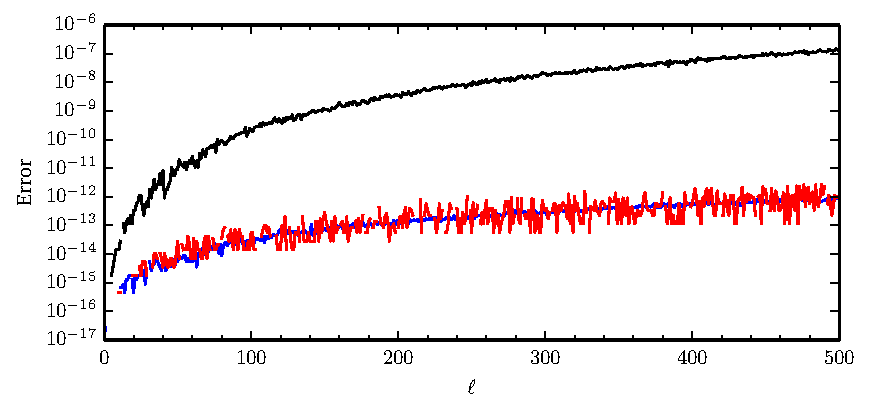
\includegraphics[width=0.9\textwidth]{figs/backmatter/SphPrecision.pdf}
 \caption[Precision of our implementation of the algorithm that evaluates the spherical harmonics]
	  {Precision of our implementation of the algorithm that evaluates the spherical harmonics. 
	  The {\color{blue} blue} curve corresponds to \eqref{eq:app.sph.sum1}, the 
	  {\color{red} red} curve to \eqref{eq:app.sph.sum2} and the black curve to 
	  \eqref{eq:app.sph.sum3}.}
 \label{fig:app.sph.precision}
\end{figure}